
\begin{flushright} {\tiny {\color{gray} \tt benchmark\_liddriven3D.tex}} \end{flushright}
%~~~~~~~~~~~~~~~~~~~~~~~~~~~~~~~~~~~~~~~~~~~~~~~~~~~~~~~~~~~~~~~~~~~~~~~~~~~~~~~~~~~~~~~~~~~~~~~~~~

It is found in \textcite{begt92} (1992). Note that simulations were carried out at a Reynolds number of 400.

The motion of the fluid is induced by moving one of the walls of a unit cube at a
constant velocity while the other walls remain stationary:
\begin{center}
\includegraphics[width=6cm]{images/benchmark_liddriven3D/setup}
\end{center}


The boundary conditions are imposed as follows:
\begin{itemize}
\item on the moving wall: $u=u_0$, $v=w=0$
\item on the symmetry plane ($y=0.5$): $v=0$
\item on the other walls: $u=v=w=0$
\end{itemize}
The lid-driven cavity problem is well suited for testing elements because of the wealth of
numerical results available.

In order to compare the computed velocity fields with published data, the usual graph of the
horizontal velocity profile $u vs z$ at the plane of symmetry was plotted.
\begin{center}
\includegraphics[width=8cm]{images/benchmark_liddriven3D/res1}
\includegraphics[width=8cm]{images/benchmark_liddriven3D/res2}\\
{\captionfont Left: results obtained with various elements against the 
solution obtained by \textcite{rota87}; 
Right: results obtained with various elements against the 
solution obtained by \textcite{redd82}.} 
\end{center}
